\chapter{System Evaluation}
\label{ch:evaluation}

This chapter evaluates the pipeline against the objectives of
Chapter~\ref{ch:introduction}, presenting internal MIMIC-IV results and the
external eICU-CRD validation, and critically discussing strengths, weaknesses,
and threats to validity.

\section{Benchmarking on the Incident-Onset Task (SQ3)}
Table~\ref{table:bench} reports discrimination at the hour-six landmark for
incident onset within 12\,h. The rule-based scores are non-discriminative to
inverse, whereas the statistical landmark models clearly exceed them, answering
SQ3 on internal data and supporting contribution~C3.

\begin{table}[h!]
    \centering
    \begin{tabular}{p{9cm}|p{3cm}}
        \hline
        \textbf{Model / Score} & \textbf{AUROC} \\
        \hline\hline
        SOFA at hour 6                              & 0.36 (inverse) \\
        qSOFA at hour 6                             & 0.49 \\
        SIRS at hour 6                              & 0.59 \\
        Multivariable logistic + trajectory slopes & 0.755 \\
        Full-feature elastic-net nomogram (C1)     & \textbf{0.775} \\
        \hline
    \end{tabular}
    \caption{Discrimination at the hour-six landmark (incident onset within
    12\,h) on MIMIC-IV.}
    \label{table:bench}
\end{table}

The trajectory-slope terms add statistically significant signal over the static
model (DeLong $p \approx 3\times10^{-7}$), supporting SQ2: modelling short-term
trajectories improves early detection over a single-time-point model.

\section{Assumption Testing (SQ1)}
The global Schoenfeld residual test rejects proportional hazards for the static
onset Cox model, so the null hypothesis of SQ1 is rejected and a time-varying
Cox model is fitted in response, satisfying contribution~C2. This confirms, on
MIMIC-IV, the non-proportionality that Kasal \emph{et al.} \cite{kasal2004cox}
reported elsewhere, and demonstrates the value of reporting, and acting on,
a diagnostic step that the MIMIC-IV Cox literature routinely omits.

\section{Real-Time Behaviour and Honest Ceilings}
Table~\ref{table:tiers} summarises the deployable model and its supporting
analyses. Two results are deliberately framed as characterisations rather than
performance wins: the strongest nomogram predictors are missingness indicators
(C4), and the PhysioNet utility is modest because the onset label is itself
gated by clinician recognition, an intrinsic ceiling rather than a model deficiency.

\begin{table}[h!]
    \centering
    \begin{tabular}{p{3.4cm}|p{8.6cm}}
        \hline
        \textbf{Component} & \textbf{Headline result (internal MIMIC-IV)} \\
        \hline\hline
        Nomogram      & AUROC 0.775; ``was-measured'' indicators dominate (C4) \\
        Supermodel    & Hourly-updating risk; AUROC 0.65--0.77 across landmarks \\
        GEE / TV-Cox  & Within-patient correlation 0.68; cluster-robust SE up to $4.5\times$ naive \\
        Utility       & Normalised utility 0.29; 90\% sensitivity gives 6.5 false alarms/patient-day \\
        Subgroups     & Calibration ratio 0.94--1.06 across sex and age \\
        GBTM          & Three latent SOFA-trajectory classes; steepest-worsening $\sim 5\times$ mortality hazard \\
        Causal        & Early antibiotics ($\le 3$\,h) associated with lower mortality across PSM/IPW/AIPW/DR \\
        \hline
    \end{tabular}
    \caption{Real-time model and supporting analyses on internal MIMIC-IV.}
    \label{table:tiers}
\end{table}

\section{External Validation on eICU-CRD (SQ3, G3)}
The frozen nomogram was applied without any refitting to 113{,}597 at-risk eICU
stays across more than 200 US ICUs (4{,}782 incident onsets within 12\,h of the
hour-six landmark). Table~\ref{table:external} reports the result against the
MIMIC development performance and an internal eICU refit ``ceiling''.

\begin{table}[h!]
    \centering
    \begin{tabular}{p{7.5cm}|p{2.5cm}|p{2.5cm}}
        \hline
        \textbf{Metric} & \textbf{eICU} & \textbf{MIMIC} \\
        \hline\hline
        AUROC (frozen transport)             & \textbf{0.686} & 0.775 \\
        \phantom{AUROC} 95\% confidence interval & [0.678, 0.694] & --- \\
        AUROC (internal eICU refit ceiling)  & 0.712 & --- \\
        Calibration slope                    & 0.54  & 1.00 \\
        Mean predicted vs.\ observed risk    & 0.121 / 0.042 & --- \\
        Brier (frozen $\rightarrow$ recalibrated) & 0.052 / 0.040 & 0.059 \\
        \hline
    \end{tabular}
    \caption{External validation of the frozen Tier-1 nomogram on eICU-CRD.}
    \label{table:external}
\end{table}

Discrimination transports with modest degradation: the frozen model (0.686) sits
close to what an eICU-native refit achieves at all (0.712), so most of the drop
from MIMIC's 0.775 reflects a harder, more heterogeneous multi-centre population
rather than model failure. The model is miscalibrated on eICU: it
over-predicts risk roughly threefold, consistent with a slope of 0.54 and the
lower onset base rate. However, a single-parameter intercept-and-slope
recalibration corrects this, reducing the Brier score from 0.052 to 0.040.
Figure~\ref{image:calibration} shows the frozen and recalibrated calibration
curves. One cross-dataset adaptation is required and reported honestly: because
eICU captures microbiology for only about 1.5\% of stays (versus antibiotics for
about 83\%), suspected infection is triggered on antibiotics alone, with a
culture used only to refine timing when present. This is a property of eICU's
data capture, not of the model.

\begin{figure}[h!]
    \centering
    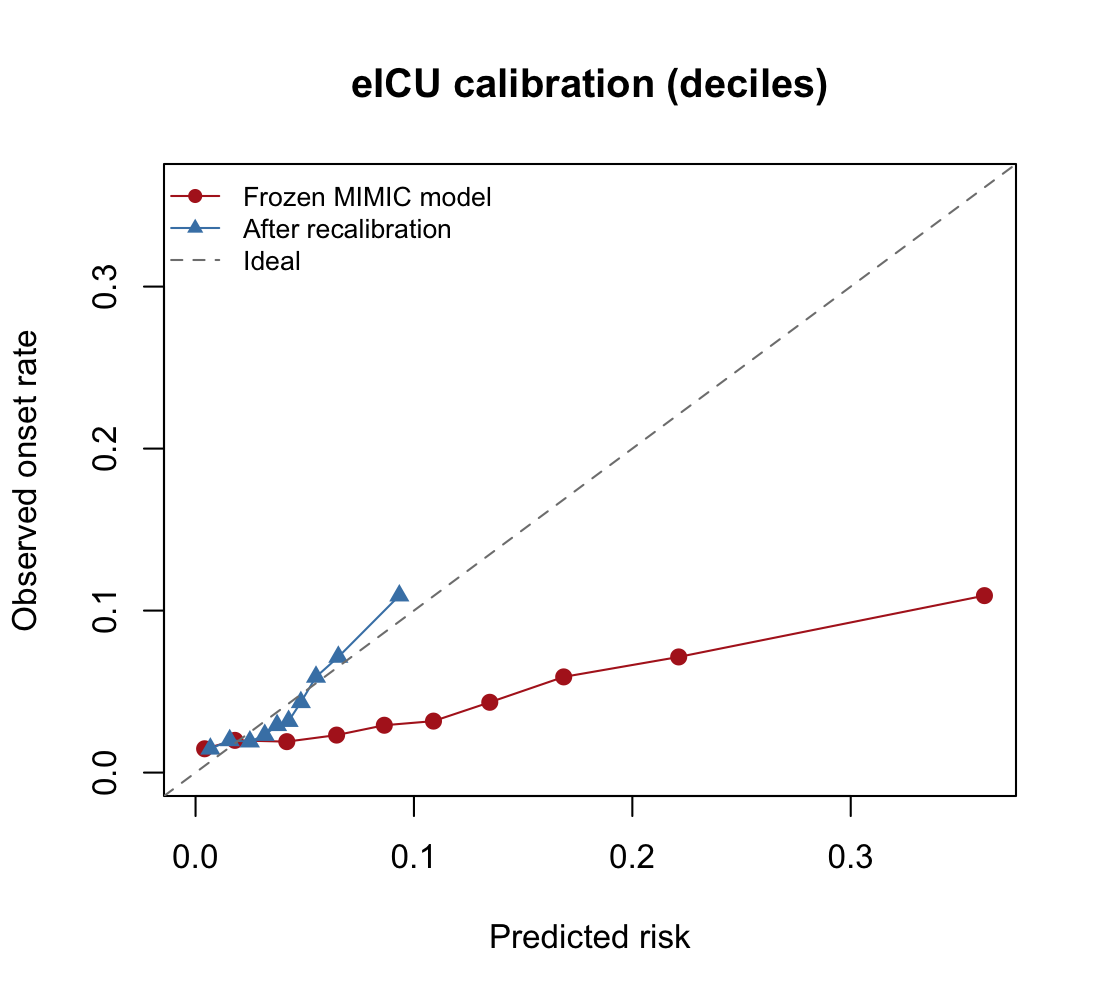
\includegraphics[width=0.7\textwidth]{images/calibration_eicu.png}
    \caption{eICU calibration by risk decile: the frozen MIMIC model
    over-predicts (below the diagonal), and a single-parameter recalibration
    restores agreement with observed onset rates.}
    \label{image:calibration}
\end{figure}

\section{Discussion and Threats to Validity}
The central empirical finding is that the ceiling on incident-onset prediction
is set by the label's dependence on clinician recognition (when cultures and
antibiotics are ordered) rather than by model class. This is why the strongest
predictors are missingness indicators and why a purely statistical model is
competitive with more complex approaches: no neural network is required to
approach a ceiling imposed by the labelling process itself. This result aligns
with, and sharpens, the informative-missingness literature
\cite{groenwold2020missingness,singh2021missingness}.

Several threats to validity remain. The onset label depends on documentation
timing; the assumed-zero SOFA baseline may slightly overcount organ dysfunction;
qSOFA uses mean arterial pressure as a proxy for systolic pressure; and the
time-varying Cox and trajectory analyses use sampled subsets for tractability.
The external validation, while confirming transportable discrimination, inherits
the antibiotic-based suspicion definition noted above. These are documented
rather than hidden, in keeping with the honest-characterisation posture of the
thesis.
